\section{Short recap of the paper}

In order to understand what the reproducibility project involves, we first start with a quick review of what has been done in the original paper. In figure \ref{fig:gan_framework}, an overview of the full 3D framework is given \cite{chan2022efficient}. The process can be split up in several steps, which will shortly be explained in this section.

\begin{figure}[H]
\centering
  \centering
  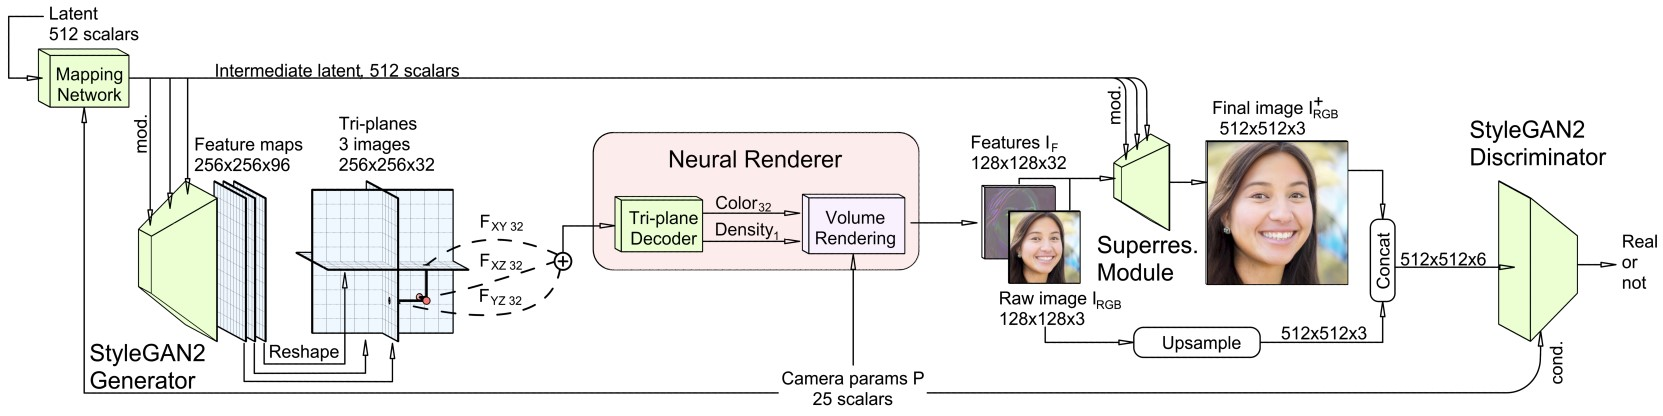
\includegraphics[width=1\linewidth]{3D GAN network.jpg}
  \caption{3D GAN framework used in the original paper \cite{chan2022efficient}}
  \label{fig:gan_framework}
\end{figure}

\begin{enumerate}
    \item \textbf{StyleGAN2-based feature generator}
    One of the advances in the paper was the decoupling of the neural rendering step from the feature generation, allowing the use of established 2D image CNNs. Here, StyleGAN2 is used, a network with a well-understood and efficient architecture that allows for style-mixing and latent-space interpolation. With the network and the camera pose parameters, features are extracted from 2D images.
    
    \item \textbf{Novel tri-plane 3D representation}
    Then, a hybrid implicit-explicit tri-plane representation such as in figure \ref{fig:triplane} is used to represent the found features. Neural implicit representations (NeRF) use fully connected layers with positional encoding, which is slow to query. Explicit voxels are fast to query, but suffer from poor scalability with regard to resolution. The combination of both, using a tri-plane, offers best of both worlds: it is fast and efficient. 

\begin{figure}[H]
    \centering
    \centering
    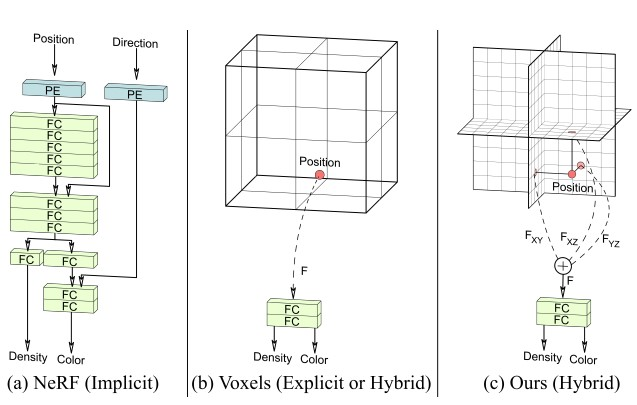
\includegraphics[width=0.5\linewidth]{triplane.jpg}
    \caption{Different types of feature representations \cite{chan2022efficient}}
    \label{fig:triplane}
\end{figure}

    \item \textbf{Neural volume renderer}
    A multi-layer perceptron (MLP) decoder reads out the 3D feature volume by sending out rays along which a certain amount of samples are taken. The output is a density $\sigma$ together with a 32-channel feature. With this information, 2D feature images are created.  
    
    \item \textbf{Super resolution module}
    Although the tri-plane representation allows for a speed-up, it is still too slow to train or render at higher resolutions. Therefore, a lower resolution of 128$^2$ pixels is rendered, after which the extra module is used to upsample to a higher resolution of 512$^2$ pixels.
    
    \item \textbf{StyleGAN2 discriminator with dual discrimination}
    Finally, an upgraded version of the standard StyleGAN2 discriminator is used. The camera pose from which the image is rendered is also fed to the discriminator, to make the generator effectively learn 3D priors. The dual discrimination is formed by concatenating the output image of the super resolution module with a bilinearly upsampled image. The two images together form a six-channel image instead of the regular three-channel image that is used by traditional GAN discriminators. The benefit is that multi-view inconsistency issues are resolved.
    
\end{enumerate}